\chapter{Metodi di upscaling}
Con il termine \emph{upscaling} si intende inferire informazioni "a scala più grande": in questo contesto significa predire il numero di specie presenti a scale più grandi di quelle che, per motivi pratici, possono essere indagate sperimentalmente e di cui si hanno dunque dati certi. Pendiamo ad esempio la foresta Amazzonica, la sua estensione è talmente vasta che è possibile campionare solamente una piccolissima percentuale di essa ($p^*=0.00016 \%$)\cite{Tovoe1701438}.\\
In questa sezione vediamo in dettaglio come è possibile ricostruire la biodiversità di un intero ecosistema a partire da un campione ridotto di SAD, occupandoci del caso in cui ad essere studiata è una frazione dell'area totale del sistema in esame.\\
Analizzeremo prima due metodi parametrici, quello della binomiale negativa e della distribuzione logaritmica di Fisher \cite{Tovoe1701438}, e poi un metodo non parametrico, quello dello stimatore di $Chao_\emph{wor}$\cite{Chaowor}.

\subsubsection{Ipotesi sul metodo di upscaling}
Nella nostra analisi assumiamo che la probabilità \emph{p} che un individuo si trovi all'interno di una zona \emph{a} contenuta in una regione \emph{A} sia proporzionale all'area della zona stessa: \emph{p}=\emph{a}/\emph{A}. Ci riferiamo a quest'ipotesi con il nome di \emph{ipotesi di campo medio}. Una conseguenza di ciò è che campionare una frazione \emph{p} di un'area \emph{A} in cui ogni individuo viene catalogato in una lista in base alla specie di appartenenza è equivalente a campionare la stessa frazione \emph{p} degli individui sulla lista. Questa è l'unica procedura imparziale che può essere adottata quando non si hanno informazioni né sulle posizioni degli individui né sulle correlazioni spaziali. Per ritenere quest'ipotesi soddisfatta bisogna verificare che la regione in esame non presenti forti disomogeneità e anisotropie, altrimenti alcune specie tenderebbero ad abitare habitat specifici all'interno della regione e dunque l'assunzione di avere una distribuzione spazialmente omogenea degli individui non sarebbe più valida.\\
%(spiegare che il modello nasce in ambito ecologico)\\
%(come viene fatto il campionamento)\\
%(parlare in generale, numero di singleton, specie rare)\\
%(metodo di Chao??)\\
\\

\section{Metodo della binomiale negativa}
%Il quadro analitico all'interno del quale si svolge questo lavoro è bastato sui seguenti passaggi:
%\begin{itemize}
  %  \item Campionare una frazione $\emph{p}^*$ dell'intera foresta e ottenere il vettore delle abbondanze delle $S^*$ specie campionate, $\emph{n}_{\emph{p}^*}={\emph{n}_1,\emph{n}_2,...,\emph{n}_{S^*}}$
  % \item Usare una combinazione lineare di binomiali negative con lo stesso $\hat \xi_{\emph{p}^*}$ e diversi valori di \emph{r} per fittare la SAD sperimentale al desiderato grado di accuratezza.
%\end{itemize}
%Di seguito analizzeremo in dettaglio le proprietà e i passaggi che ci permettono di ottenere le informazioni desiderate.\\
Quando facciamo\emph{ upscaling} siamo interessati alla SAD ed al numero totale di specie presenti a scala globale, cioè in tutta l'area \emph{A} dell'ecosistema in esame.
Denotiamo con $P(\emph{n}|1)$ la probabilità che una specie abbia esattamente \emph{n} individui a scala globale (con il numero 1 si intende l'intero ecosistema), anche nota come \emph{abbondanza relativa delle specie} (RSA).
Notiamo che P(\emph{n}|1) deve essere definita solamente per $\emph{n}\ge1$ poiché per poter osservate una data specie questa deve essere popolata da almeno un individuo.\newline
In questo metodo di \emph{upscaling} si ipotizza che la SAD segua una distribuzione binomiale negativa $\mathcal{P}(\emph{n}|\emph{r},\xi)$ di parametri (\emph{r},$\xi$):
\\ 
\begin{equation}
 P(\emph{n}|1)=\emph{c}(\emph{r},\xi)\mathcal{P}(\emph{n}|\emph{r},\xi)
 \label{eq:NBfunctform}
\end{equation}
con 
\begin{equation}
    \mathcal{P}(\emph{n}|\emph{r},\xi)=\binom{n+\emph{r}-1}{n}\xi^n(1-\xi)^{\emph{r}}     
\end{equation}
e
\begin{equation}
     \emph{c}(\emph{r},\xi)=\frac{1}{1-(1-\xi)^{\emph{r}}}
\end{equation}
\\ 
dove \emph{c} è la costante di normalizzazione.
Quest'ultima è stata calcolata imponendo \newline  $\sum_{\emph{n}=1}^\infty P(\emph{n}|1)=1$, dove la somma parte da 1 poiché  non si possono osservare specie con abbondanza nulla.
Notiamo che invece $\mathcal{P}(\emph{n}|\emph{r},\xi)$è normalizzata per $\emph{n}\ge0$: questo perché nei campioni esiste una probabilità non nulla di che una specie presente nell'intero ecosistema abbia \emph{n}=0 individui. Dunque in questo modo si tiene conto del numero di specie mancanti nei campioni.\\
Consideriamo ora un campione di area \emph{a} e definiamo \emph{p}=\emph{a}/\emph{A} la scala del campione, cioè la frazione di ecosistema osservato.
Come primo passaggio calcoliamo la RSA del campione assumendo che quest'ultima non sia influenzata da correlazioni spaziali. Quest'ipotesi è ben soddisfatta ed è stata verificata usando dati di foreste generati \emph{in silico} a vari gradi di correlazione spaziale\cite{Tovoe1701438}.\\
Sotto queste ipotesi la probabilità che una specie presenti \emph{k} individui in un'area \emph{a=pA}, condizionata dal fatto che presenta \emph{n} individui nella regione totale \emph{A} è data dalla distribuzione binomiale:
\\ 
\begin{equation}
\mathcal{P}_\emph{binom}(\emph{k}|\emph{n},\emph{p})=\begin{cases} \binom{\emph{n}}{\emph{k}}\emph{p}^\emph{k}(1-\emph{p})^{\emph{n-k}} & \mbox{se }\emph{k}=0,...,\emph{n} \\ 0 & \mbox{se }\mbox{\emph{k>n}}
\end{cases}
\end{equation}
\\ 

Infatti, in assenza di correlazioni spaziali, la probabilità che uno degli individui di una specie si trovi in una regione di area \emph{a} è esattamente \emph{p}.

Mostriamo ora un risultato chiave per il metodo di upscaling:
\subsection{Proprietà di invarianza per forma 
della distribuzione binomiale negativa}
Sia $ P(\emph{n}|1)=\emph{c}(\emph{r},\xi)\mathcal{P}(\emph{n}|\emph{r},\xi) $ la RSA dell'ecosistema a scala globale e denotiamo con $\mathcal{P}(\emph{k}|\emph{n},\emph{p})$ la probabilità che una specie abbia abbondanza \emph{k} alla scala \emph{p}$\in$(0,1) condizionata dal fatto che alla scala globale \emph{A} sono presenti \emph{n} individui di quella specie.
Se $\mathcal{P}(\emph{k}|\emph{n,p})=\mathcal{P}_\emph{binom}(\emph{k}|\emph{n},\emph{p})$ segue una distribuzione binomiale, allora la RSA $\mathcal{P}_\emph{sub}(\emph{k}|\emph{p})$ alla scala di campionamento \emph{p} è ancora una binomiale negativa per $\emph{k}\ge1$ con il parametro $\xi$ riscalato e lo stesso \emph{r}:
\\ \\
\begin{equation}
    \mathcal{P}_\emph{sub}(\emph{k}|\emph{p})=\begin{cases} \emph{c}(\emph{r},\xi)\mathcal{P}(\emph{k}|\emph{r},\hat \xi_\emph{p}), & \mbox{ }\emph{k}\ge1 \\ 1-\emph{c}(\emph{r},\xi)/\emph{c}(\emph{r},\hat\xi_{\emph{p}}), & \mbox{ }\mbox{\emph{k=0}}
    \end{cases}
\label{eq:RSAbinom}
\end{equation}

con 
\begin{equation}
    \hat\xi_{\emph{p}}=\frac{\emph{p}\xi}{1-\xi(1-\emph{p})}.
\label{eq:NBparametersub}
\end{equation}
Infatti la probabilità $\mathcal{P}_{sub}(\emph{k}|\emph{p})$ di trovare una specie popolata da $\emph{k} \ge 0$ individui nel campione di area \emph{a}=\emph{p}\emph{A} è:
%\begin{proof}

\begin{equation}
   % \begin{aligned}
  %  A & = B + C\\
  %    & = D + E + F\\
   %   & = G
  %\end{aligned}
  \begin{aligned}
   \emph{k}\ge 1: \mathcal{P}_\emph{sub}(\emph{k}|\emph{p}) & = \sum_{\emph{n}\ge \emph{k}}\mathcal{P}_\emph{binom}(\emph{k}|\emph{n},\emph{p})P(\emph{n}|1)\\
      & = \sum_{\emph{n}\ge \emph{k}} \binom{\emph{n}}{\emph{k}}\emph{p}^\emph{k}(1-p)^{\emph{n}-\emph{k}} \cdot\emph{c}(\emph{r},\xi) \binom{\emph{n}+\emph{r}-1}{\emph{n}}\xi ^ \emph{n}(1-\xi)^\emph{r}\\
      & =\emph{c}(\emph{r},\xi)\binom{\emph{k}+\emph{r}-1}{\emph{k}}\left( \frac{\emph{p}\xi}{1-\xi(1-\emph{p})} \right)^\emph{k}\left( \frac{1-\xi}{1-\xi(1-\emph{p})} \right)^\emph{r} \\
      & = \emph{c}(\emph{r},\xi)\binom{\emph{k}+\emph{r}-1}{\emph{k}} \hat \xi_\emph{p}^\emph{k}(1-\hat \xi_\emph{p})^\emph{r} = \emph{c}(\emph{r},\xi)\cdot \emph{P}(\emph{k}|\emph{r},\hat \xi_\emph{p})
  \end{aligned}
\end{equation}

dove abbiamo usato la (\ref{eq:NBparametersub}) per $\hat \xi_\emph{p}$ per la penultima uguaglianza, e

 \begin{equation}
     \begin{aligned}
         \emph{k}=0: \mathcal{P}_\emph{sub}(0|\emph{p}) & =1-\sum_{\emph{n}\ge\emph{1}}\mathcal{P}_\emph{sub}(\emph{k}|\emph{p}) \\
         &=1-\sum_{\emph{n}=1}^\infty \emph{c}(\emph{r},\xi)\cdot \binom{\emph{k}+\emph{r}-1}{\emph{k}}\hat \xi_\emph{p}^\emph{k}(1-\hat \xi_\emph{p})^\emph{r}\\
         &=1-\emph{c}(\emph{r},\xi)\cdot \sum_{\emph{k}=1}^\infty \mathcal{P}(\emph{k}|\emph{r},\hat \xi _\emph{p})=1-\frac{\emph{c}(\emph{r},\xi)}{\emph{c}(\emph{r}, \hat \xi_\emph{p})}.
     \end{aligned}
 \end{equation}
 
%\end{proof}
 
\subsection{Il numero di specie a scala globale}
Ricordiamo che questo metodo fa uso solamente delle informazioni che si possono ottenere da un campione ad una certa scala $p^*$, infatti noi abbiamo informazioni solo sulle abbondanze delle $S^*\le S$ specie presenti nel campione esaminato. Denotando il numero di specie di abbondanza \emph{k} alla scala $p^*$ con $S^*(\emph{k})$, otteniamo, per $\emph{k}\ge 1$:

\begin{equation}
    \frac{S^*(\emph{k})}{S^*}\equiv P(\emph{k}|\emph{p}^*)=\frac{\mathcal{P}_\emph{sub}(\emph{k}|\emph{p}^*)}{\sum_{k^{'} \ge 1}^{} \mathcal{P}_\emph{sub}(\emph{k}^{'}|\emph{p}^{*})}
    =\frac{\mathcal{P}(\emph{k}|\emph{r},\hat\xi_{\emph{p}^*})}{\sum_{k^{'} \ge 1}^{} \mathcal{P}(\emph{k}^{'}|\emph{r},\hat \xi_{\emph{p}^*})}
    =\emph{c}(\emph{r},\hat\xi_{\emph{p}^*})\mathcal{P}(\emph{k}|\emph{r},\hat \xi_{\emph{p}^*})
    \label{eq:SstarRSA}
\end{equation}

che, dalla (\ref{eq:NBfunctform}), è una binomiale negativa normalizzata per $\emph{k}\ge 1$, mentre $\mathcal{P}(\emph{k}|\emph{r},\hat \xi_{\emph{p}^*})$ è normalizzata per $\emph{k}\ge 0$.
Per quanto detto sopra otteniamo dunque il seguente risultato: partendo da una distribuzione binomiale negativa per la RSA a scala globale, anche la RSA a scala ridotta risulta distribuita secondo una binomiale negativa di parametri lo stesso \emph{r} e $\hat \xi_\emph{p}^*$ riscalato.
Una RSA avente la proprietà di avere la stessa forma funzionale a scale differenti è detta essere \emph{invariante per forma}.

Fittando la RSA dei dati alla scala $\emph{p}^*$ possiamo dunque trovare i parametri \emph{r} e $\hat \xi_\emph{p}^*$ e, invertendo l'equazione (\ref{eq:NBparametersub}), troviamo:
\begin{equation}
    \xi=\frac{\hat \xi_{\emph{p}^*}}{\emph{p}^*+\hat \xi_{\emph{p}^*}(1-\emph{p}^*)}.
\label{eq:NBparameter}
\end{equation}
Usando ancora la (\ref{eq:NBparametersub}) per eliminare $\xi$ dall'ultima equazione, otteniamo la seguente relazione per il parametro $\xi$ alle due scale \emph{p} e $\emph{p}^*$:
\begin{equation}
    \hat\xi_\emph{p}=\frac{p \hat \xi_{\emph{p}^*}}{\emph{p}^*+\hat\xi_{\emph{p}^*}(\emph{p}-\emph{p}^*)}\equiv U(\emph{p},\emph{p}^*|\hat \xi_{\emph{p}^*})
    \label{eq:xihatp}
\end{equation}
dalla quale, ovviamente, è possibile riottenere sia la (\ref{eq:NBparametersub}) che la (\ref{eq:NBparameter}) ponendo $\xi \equiv \hat \xi_{\emph{p}=1} $.

Vogliamo ora determinare la relazione tra il numero totale di specie S alla scala globale \emph{p}=1 e il numero totale di specie osservate localmente $S_\emph{p}$ alla scala \emph{p}.
D'ora in avanti per denotare il numero di specie alla scala locale useremo la notazione $S^*\equiv S_{\emph{p}^*}$.
Notiamo che:
\begin{equation}
\mathcal{P}_\emph{sub}(\emph{k=0}|\emph{p}^*)=\frac{S-S^*}{S}
\end{equation}
\begin{equation}
    \mathcal{P}_\emph{sub}(\emph{k}|\emph{p}^*)=\frac{S^*(\emph{k})}{S}.
\end{equation}
Usando la seconda delle (\ref{eq:RSAbinom}), il numero di specie presenti nell'intera foresta è dato, in termini dei dati del campione osservato, da:
\begin{equation}
S=\frac{S^*}{1-\mathcal{P}_\emph{sub}(\emph{k}=0|\emph{p}^*)}=S^*\frac{1-(1-\xi)^r}{1-(1-\hat \xi_{\emph{p}}^*)^r}.
\label{eq:upscaleNB}
\end{equation}

Notiamo che, se si assume che la RSA segua una distribuzione binomiale negativa a scala globale, il valor medio dell'abbondanza totale riscala linearmente con l'area, infatti:
\begin{equation}
    \begin{aligned}
    \mathbb{E}(N^*) & =\sum_{\emph{k}=1}^\infty \emph{k}S \emph{c}(\emph{r},\xi)\binom{\emph{k}+\emph{r}-1}{\emph{k}}\hat \xi_{\emph{p}^*}^\emph{k}(1-\hat \xi_{\emph{p}^*})^\emph{r}=S\emph{c}(\emph{r},\xi)\emph{r}\frac{\hat \xi_{\emph{p}^*}}{1-\hat \xi_{\emph{p}^*}}\\
    & =S\emph{c}(\emph{r},\xi)\emph{r}\frac{\emph{p}\xi}{1-\xi}=\emph{p}\mathbb{E}(N)
    \end{aligned}
\end{equation}
 % \begin{aligned}
  %  A & = B + C\\
  %    & = D + E + F\\
   %   & = G
  %\end{aligned}
\section{Metodo della distribuzione logaritmica}
%Ora mostreremo che è possibile risalire al numero di specie anche quando si suppone che la SAD a scala globale sia distribuita secondo una distribuzione di Fisher.\\
Questo modello naque nei primi anni '40 quando il chimico e naturalista britannico Alexander Steven Corbet, dopo aver trascorso due anni in Malesia a studiare e catalogare le specie di farfalle, tornò in Inghilterra e mostrò i suoi dati al collega Ronald Aylmer Fisher. Corbet si chiese quante nuove specie avrebbe trovato se fosse tornato in Malesia per altri due anni. Per rispondere a questa domanda, il padre della statistica Fisher fu il primo matematico ad affrontare il problema della stima del numero di specie, che da quel momento ha trovato larghe applicazioni in vari campi scientifici. Dunque in questo contesto Fisher ha introdotto la distribuzione che da lui prende nome e che viene molto utilizzata in teoria dell'ecologia per descrivere la RSA di un ecosistema, ovvero la distribuzione logaritmica di parametro \emph{x} \cite{Fisher1943}:

\begin{equation}
P(\emph{n}|1)=P^\emph{LS}(\emph{n}|\emph{x})=\alpha(\emph{x})\frac{\emph{x}^\emph{n}}{\emph{n}}, \ \alpha(x)=-(\log(1-\emph{x}))^{-1},
\end{equation}
dove $\alpha(x)$ è la costante di normalizzazione.
Assumendo anche questa volta che la RSA del campione non sia affetta da correlazioni spaziali si trova che anche la distribuzione logaritmica, essendo un caso particolare della distribuzione binomiale negativa, soddisfa la proprietà di invarianza.

\subsection{Proprietà di invarianza per forma della distribuzione logaritmica}
Sia $P(\emph{n}|1)=\alpha(\emph{x})\mathcal{P}^{\emph{LS}}(\emph{n}|\emph{x})$ la RSA alla scala globale e denotiamo con $\mathcal{P}(\emph{k}|\emph{n},\emph{p})$ la probabilità che una specie abbia abbondanza \emph{k} nel campione alla scala \emph{p} $\in$ (0,1) condizionata dal fatto  alla scala globale \emph{A} la specie possiede \emph{n} individui.\\
Se $\mathcal{P}(\emph{k}|\emph{n,p})=\mathcal{P}_\emph{binom}(\emph{k}|\emph{n,p})$ è distribuita secondo una binomiale, allora la RSA alla scala del campione, $\mathcal{P}^\emph{LS}_\emph{sub}(\emph{k}|\emph{p})$, è ancora una distribuzione logaritmica per $\emph{k}\ge 1$ con il parametro \emph{x} riscalato:

\begin{equation}
\mathcal{P}^\emph{LS}_\emph{sub}(\emph{k}|\emph{p})=\begin{cases} \alpha(\emph{x}) \mathcal{P}^\emph{LS}(\emph{k}|\emph{$ \hat x$}_\emph{p}) & \mbox{ }\mbox{ \emph{k} } \ge 1 \\ 1-\alpha(\emph{x})/\alpha(\emph{$\hat x$}_\emph{p}) & \mbox{ } \mbox{ \emph{k}=0}
\end{cases}
\end{equation}
con



\begin{equation}
\emph{$\hat x$}_\emph{p}=\frac{\emph{px}}{1-\emph{x}(1-\emph{p})}.
\label{eq:LSparametersub}
\end{equation}

Infatti la probabilità $\mathcal{P}_\emph{sub}^\emph{LS}(\emph{k}|\emph{p})$ di trovare una specie con popolazione $\emph{k} \ge 0$ nel sotto campione di area \emph{a}=\emph{p}\emph{A} è:
\begin{equation}
    \begin{aligned}
   \emph{k} \ge 1: \mathcal{P}_\emph{sub}^\emph{LS}(\emph{k}|\emph{p}) & = \sum_{\emph{n}\ge \emph{k}} \emph{P}_\emph{binom}(\emph{k}| \emph{n},\emph{p})P(\emph{n}|1) \\
     & = \sum_{\emph{k} \ge \emph{n}} \binom{\emph{n}}{\emph{k}}\emph{p}^\emph{k}(1-\emph{p})^\emph{n-k} \cdot \alpha(\emph{x})\frac{\emph{x}^\emph{n}}{\emph{n}}\\
     & = \alpha(\emph{x})\left( \frac{\emph{px}}{1-\emph{x}(1-\emph{p})} \right)^ \emph{k} \frac{1}{\emph{k}} \\
     & = \alpha(\emph{x}) \frac{\emph{$ \hat x$}_\emph{p}^\emph{k}}{\emph{k}}=\alpha(\emph{x})\cdot\mathcal{P}^\emph{LS}(\emph{k}|\emph{$\hat x$}_\emph{p})
    \end{aligned}
\end{equation}

dove abbiamo usato la relazione (\ref{eq:LSparametersub}) nella penultima uguaglianza,e
\begin{equation}
    \begin{aligned} 
     \emph{k}=0: \mathcal{P}_\emph{sub}^\emph{LS}(0|\emph{p}) & = 1- \sum_{\emph{k} \ge 1} \emph{P}_\emph{sub}^\emph{LS}(\emph{k}|\emph{p})\\
      & = 1- \sum_{\emph{k}=1}^\infty \alpha(\emph{x}) \cdot \frac{\emph{$ \hat x$}_\emph{p}^\emph{k}}{\emph{k}}\\
     & = 1-\alpha(\emph{x}) \cdot \sum_{\emph{k}=1}^\infty \mathcal{P}^\emph{LS}(\emph{k}|\emph{$\hat x$}_\emph{p})= 1-\frac{\alpha(\emph{x})}{\alpha(\emph{$\hat x$}_\emph{p})}.
    \end{aligned}
\end{equation}


Notiamo che (\ref{eq:LSparametersub}) è analoga a (\ref{eq:NBparametersub}). Dunque l'analogo di (\ref{eq:NBparameter}) è


\begin{equation}
\emph{x}=\frac{\emph{$\hat x$}_{\emph{p}}^*}{\emph{p}^*+\emph{$\hat x$}_{\emph{p}}^*(1-\emph{p}^*)}
\label{eq:LSparameter}
\end{equation}

e l'equazione (\ref{eq:xihatp}) vale anche in questo caso.


La RSA può essere ottenuta come nell'equazione (\ref{eq:SstarRSA}) ed è data da:
\\
\begin{equation}
P(\emph{k}|\emph{p}^*)=\frac{\emph{P}^\emph{LS}_\emph{sub}(\emph{k}|\emph{p}^*)}{\sum_{k^{'} \ge 1}^{} \emph{P}^\emph{LS}_\emph{sub}(\emph{k}^{'}|\emph{p}^*)}=\alpha(\emph{$\hat x$}_{\emph{p}}^*) \frac{\emph{$\hat x$}_{\emph{p}^*}^\emph{k}}{\emph{k}}=\alpha(\emph{$\hat x$}_{\emph{p}}^*)P^\emph{LS}(\emph{n}| \emph{$\hat x$}_{\emph{p}}^*)
\end{equation}.
\\ 



\subsection{Il numero di specie a scala globale}
Il numero di specie con popolazione $\emph{k} \ge 1$ presenti nel campione di area \emph{a}=\emph{pA} è dato da:

\begin{equation}
S_\emph{p}(k) \equiv S\emph{P}_\emph{sub}^\emph{LS}(\emph{k}|\emph{p})=S\alpha(\emph{x})\frac{\emph{$\hat x$}^\emph{k}_\emph{p}}{\emph{k}}=\hat \alpha \frac{\emph{$\hat x$}^\emph{k}_\emph{p}}{\emph{k}}
\end{equation} 
\\
dove abbiamo unito le costanti S e $\alpha (\emph{x})$ in un unico termine $\hat \alpha$ che non dipende dalla scala \emph{p} del campione. Quando ci riferiremo alla scala $\emph{p}^*$ useremo, per brevità di notazione, $S^*(\emph{k})\equiv S_{\emph{p}^*}(\emph{k})$.\\
Allora il numero totale di specie $S^*$ e l'abbondanza totale $N^*$ alla scala $\emph{p}^*$ sono date rispettivamente da:

\begin{equation}
S^*=\sum_{\emph{k}=1}^\infty S^*(\emph{k})=-\hat \alpha \log (1-\emph{$\hat x$}_{\emph{p}^*})
\label{eq:SstarLS}
\end{equation}

\begin{equation}
N^*=\sum_{\emph{k}=1}^\infty \emph{k}S^*(\emph{k})=\hat \alpha \frac{\emph{$\hat x$}_{\emph{p}^*}}{1-\emph{$\hat x$}_{\emph{p}^*}}.
\label{eq:NstarLS}
\end{equation}
\\
Poiché $S^*$ e $N^*$ sono note dal campione, possiamo trovare $\hat \alpha$ risolvendo la seguente equazione:

\begin{equation}
N^*- \hat \alpha(\exp( \frac{S^*}{\hat \alpha})-1)=0,
\label{eq:solve}
\end{equation}
\\
che si ottiene inserendo l'espressione di $  \emph{$\hat x$}_{\emph{p}^*} $ da (\ref{eq:SstarLS}) nella (\ref{eq:NstarLS}).
\\ \\
Vogliamo ora dedurre le informazioni a scala globale \emph{p}=1 dai dati disponibili alla scala \emph{p}=$\emph{p}^*$. Dalle considerazioni precedenti sappiamo che $ \hat \alpha$ è un parametro indipendente dalla scala, dunque abbiamo le seguenti relazioni per S e N:

\begin{equation}
S=-\hat \alpha \log(1-\emph{x})
\label{eq:SLS}
\end{equation}

\begin{equation}
N=\hat \alpha \frac{\emph{x}}{1-\emph{x}}.
\label{eq:NLS}
\end{equation}

dalle quali otteniamo:

\begin{equation}
S=\hat \alpha \log \left (1+ \frac{N}{\hat \alpha} \right ), \ \hat \alpha=S\alpha(\emph{x}).
\label{eq:SalphaLS}
\end{equation}

Dunque per dedurre la biodiversità a scala globale, $S$, è necessaria una stima dell'abbondanza totale $N$. Prendiamo $N=N^*/ \emph{p}^*$. Notiamo che questo è consistente con il nostro quadro teorico nel quale assumiamo che la RSA sia \emph{invariante per forma}: infatti si può dimostrare che, se si assume che la RSA segua una distribuzione di Fisher a scala globale, il valor medio dell'abbondanza totale riscala linearmente con l'area:

\begin{equation}
\mathbb{E}(N^*)=\sum_{\emph{k}=1}^\infty \emph{k}S^*(\emph{k})=\sum_{\emph{k}=1}^\infty \emph{k} \hat \alpha  \frac{\hat {\emph{x}}^\emph{k}_{\emph{p}^*}}{\emph{k}}=\alpha \frac{\hat {\emph{x}}_{\emph{p}^*}}{1-\hat {\emph{x}}_{\emph{p}^*}}= \hat 	\alpha \frac{\emph{px}}{1-x}= \emph{p}^* \mathbb{E}(N),
\end{equation}
\\
dove abbiamo usato la  (\ref{eq:LSparametersub}).

Per dedurre in modo alternativo la biodiversità a scala globale, analogamente a quanto fatto per il metodo della binomiale negativa, si potrebbe usare anche la relazione seguente:

\begin{equation}
   S=\frac{S^*}{1-\emph{P}_\emph{sub}^\emph{LS}(\emph{k=0}|\emph{p}^*)}=S^*\frac{\log(1-\emph{x})}{\log(1-\emph{$\hat x$}_{\emph{p}^*})}.
   \label{eq:upscalingLS}
\end{equation}

In questo caso non bisogna avere una stima del numero totale di individui $N$ nell'area \emph{A}. È stato verificato su dati riguardanti la biodiversità nelle foreste che i due metodi restituiscono previsioni equivalenti\cite{Tovoe1701438}.

\begin{figure}
\centering
  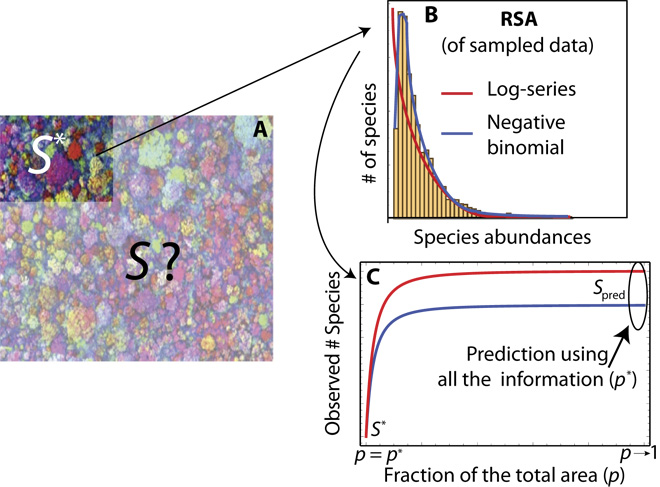
\includegraphics[width=0.6\linewidth]{Figure/RSA.jpg}
  \caption{\textbf{Rappresentazione schematica del modello di upscaling}. Questo consiste in tre passaggi. (\textbf{A}) Conosciamo l'abbondanza di $S^*$ specie alla scala di campionamento $\emph{p}^*$. (\textbf{B}) Facciamo un fit della SAD con una binomiale negativa o una distribuzione logaritmica. (\textbf{C}) Usando i parametri del miglior fit ottenuti in (B) e usando le equazioni (\ref{eq:SalphaLS}) e (\ref{eq:upscaleNB}) per dedurre la biodiversità dell'intero ecosistema.\cite{Tovoe1701438} }
  \label{fig:RSA1}
\end{figure}


\section{Metodo $Chao_\emph{wor}$}
Introduciamo ora il metodo non parametrico sviluppato da Chao, nato nell'ambito di uno schema di campionamento senza reinserimento. Il pedice \emph{wor} sta infatti per "\emph{without repetition}". Questo è il sistema di indagine più usato quando si devono campionare individui che non si desidera osservare ripetutamente (ad esempio nello studio delle foreste, nel quale gli alberi vengono censiti in piccole aree che sono selezionate senza ripetizione). In questo schema di campionamento ogni individuo o ogni unità di campionamento possono essere indagati una sola volta.\\
Assumiamo che in un ecosistema ci siano $S$ specie indicizzate da 1 a $S$.
Sia $N_\emph{i}$ (abbondanza assoluta) il numero di individui appartenenti alla \emph{i}-esima specie, \emph{i}=1,...,S, e $N_\emph{i}>0$. La popolazione totale dunque è data da $N=\sum_{\emph{i}=1}^{S} N_\emph{i}$. Assumiamo che la dimensione del campione $N$ sia nota, e che quindi sia nota anche la frazione di campionamento.\\
Supponiamo di prendere dall'intero ecosistema un campione di $N^*$ individui, campionandoli senza reinserimento. Sia $X_\emph{i}$ la frequenza della specie campionata cioè il numero di individui della \emph{i}-esima specie osservati nel campione. Solo le specie con  $X_\emph{i}>0$ sono osservabili nel campione. Sia $S^*_\emph{k}$ il numero di specie nel campione che sono rappresentate esattamente da \emph{k} individui, dunque $S^*_0$ denota il numero di specie che non sono state osservate nel campione. Dunque abbiamo che $\emph{n}=\sum_{\emph{i}=1}^S X_\emph{i}=\sum_{\emph{k}>1} \emph{k}S^*_\emph{k}$.
Definiamo $\emph{p}^*=N^*/N$ la frazione di campionamento e $S^*$ il numero di specie osservate nel campione, $S^*=\sum_{\emph{k>1}} S^*_\emph{k}$.\\
Generalmente la probabilità che una specie venga rilevata, o rate di rilevamento, dipende sia dall'abbondanza della specie nel campione sia da caratteristiche specifiche degli individui come ad esempio il modo di spostarsi e muoversi all'interno dell'ambiente, colore, forma e dimensione.\\ Consideriamo dunque il caso generale in cui la probabilità di trovare un individuo possa variare a seconda della specie di appartenenza e indichiamola con $\theta_\emph{i}>0$ per la \emph{i}-esima specie.
Sotto queste ipotesi, definendo $\emph{p}_\emph{i}=N_\emph{i}/N $ come l'abbondanza relativa, il rate di rilevamento per la \emph{i}-esima specie diventa $\psi_{\emph{i}}=\frac{N_\emph{i}\theta_\emph{i}}{\sum_{\emph{k}=1}^S N_\emph{k}\theta_\emph{k}}=\frac{\emph{p}_\emph{i}\theta_\emph{i}}{\sum_{\emph{k}=1}^S \emph{p}_\emph{k}\theta_\emph{k}}$ con $\emph{i}=1,...,S$.
Intuitivamente, il numero di individui che hanno la stessa possibilità di essere osservati è dato da $N_\emph{i}\psi_\emph{i}$, ma poiché questo potrebbe essere un numero non intero, definiamo una variabile a valori interi $Z_\emph{i}$, che rappresenta il numero di individui che hanno la stessa possibilità di essere osservati per la \emph{i}-esima specie. Siccome $Z\ge 1$ e la frazione di individui campionata è $\emph{n}/N$, si può modellare il vettore \textbf{Z}=($Z_1,Z_2,...,Z_S$) attraverso una distribuzione multinomiale troncata di parametri N e  ($\psi_1^*,\psi_2^*,...,\psi_S^*$), dove $\psi_\emph{i}^* = \psi_i / P  \left\{\emph{z}:\emph{z}_\emph{i} \ge 1 , \emph{i}=1,...,S \right\} $, \textbf{z}=($\emph{z}_1 , \emph{z}_2,...,\emph{z}_S$) e $\sum_{\emph{i}=1}^S \emph{z}_\emph{i}=N$. Per ogni dato valore di \textbf{z}=($\emph{z}_1 , \emph{z}_2,...,\emph{z}_S$), le frequenze con cui appaiono gli individui della specie \emph{i}-esima nel campione, ($X_1,X_2,...,X_S$), seguono una distribuzione ipergeometrica generalizzata:
\\ \\
\begin{equation}
    P(X_\emph{i}=\emph{x}_\emph{i}, \emph{i}=1,2,...,S)=\binom{\emph{z}_1}{\emph{x}_1}\binom{\emph{z}_2}{\emph{x}_2}...\binom{\emph{z}_S}{\emph{x}_S}/\binom{N}{\emph{n}}
\end{equation}
$$ \emph{z}_\emph{i}\ge 1, \\ \sum_{\emph{i}=1}^S \emph{z}_\emph{i}=N.$$

Sulla base di questo modello generale, la distribuzione marginale per ognuna delle frequenze con le quali vengono individuate le specie è una distribuzione ipergeometrica:
\begin{equation}
P(X_\emph{i}=\emph{x}_\emph{i})=\binom{\emph{z}_\emph{i}}{\emph{k}}\binom{N-\emph{z}_\emph{i}}{\emph{n}-\emph{k}}/\binom{N}{\emph{n}}.
\label{eq:multinomial}
\end{equation}

\subsection{Il numero di specie a scala globale}
Vediamo dunque com'è possibile dedurre, sotto queste ipotesi, il numero di specie a scala globale a partire da un vettore di abbondanze ottenuto esaminando una frazione dell'intero ecosistema.\\ \\
Il valore di aspettazione per i contatori di frequenze $S^*_\emph{k}$ usando la (\ref{eq:multinomial}) è:
\begin{equation}
    \mathbb{E}(S^*_\emph{k})=\sum_\emph{i}^S P(X_\emph{i}=\emph{k})= \sum_{\emph{i}=1}^S \binom{\emph{z}_\emph{i}}{\emph{k}}\binom{N-\emph{z}_\emph{i}}{\emph{n}-\emph{k}}/\binom{N}{\emph{n}}
    \label{eq:expectationvalue}
\end{equation}

In particolare:
$$\mathbb{E}(S^*_0)=\sum_{\emph{i}=1}^S \binom{N-\emph{z}_\emph{i}}{\emph{n}}/\binom{N}{\emph{n}}$$

$$ \mathbb{E}(S^*_1)=\sum_{\emph{i}=1}^S \binom{\emph{z}_\emph{i}}{1} \binom{N-\emph{z}_\emph{i}}{\emph{n}-1}/\binom{N}{\emph{n}}=\sum_{\emph{i}=1}^S\frac{\emph{n}\emph{z}_\emph{i}}{N-\emph{z}_\emph{i}-\emph{n}+1} \binom{N-\emph{z}_\emph{i}}{\emph{n}}/\binom{N}{\emph{n}}$$



$$ \mathbb{E}(S^*_2)=\sum_{\emph{i}=1}^S \binom{\emph{z}_\emph{i}}{2} \binom{N-\emph{z}_\emph{i}}{\emph{n}-2}/\binom{N}{\emph{n}}=\sum_{\emph{i}=1}^S\frac{\emph{n}(\emph{n}-1)\emph{z}_\emph{i}(\emph{z}_\emph{i}-1)}{2(N-\emph{z}_\emph{i}-\emph{n}+1)(N-\emph{z}_\emph{i}-\emph{n}+2)} \binom{N-\emph{z}_\emph{i}}{\emph{n}}/\binom{N}{\emph{n}}$$

Per la disuguaglianza di Cauchy-Schwarz si ha:

$$
\left \{ \sum_{\emph{i}=1}^S\frac{\emph{n}\emph{z}_\emph{i}}{N-\emph{z}_\emph{i}-\emph{n}+1} \binom{N-\emph{z}_\emph{i}}{\emph{n}}/\binom{N}{\emph{n}} \right \}^2 \le $$ 
$$ \left \{ \sum_{\emph{i}=1}^S \binom{N-\emph{z}_\emph{i}}{\emph{n}}/\binom{N}{\emph{n}} \right \}\times \left \{ \sum_{\emph{i}=1}^S \left(\frac{\emph{n}\emph{z}_\emph{i}}{N-\emph{z}_\emph{i}-\emph{n}+1}\right)^2 \binom{N-\emph{z}_\emph{i}}{\emph{n}}/\binom{N}{\emph{n}} \right \},
$$
 dove vale il segno di uguaglianza quando tutte le $\emph{z}_\emph{i}$ sono uguali.
 
 La parte sinistra della disuguaglianza è $ \left \{ \mathbb{E}(S^*_1) \right \}^2$ e la prima sommatoria della parte destra è $ \left \{ \mathbb{E}(S^*_0) \right \}$. Per quanto riguarda la seconda sommatoria di destra riscrivendo:
 
 $$\left(\frac{\emph{n}\emph{z}_\emph{i}}{N-\emph{z}_\emph{i}-\emph{n}+1}\right)^2=\frac{\emph{n}}{\emph{n}-1}\left(\frac{\emph{n}(\emph{n}-1)\emph{z}_\emph{i}(\emph{z}_\emph{i}-1)}{(N-\emph{z}_\emph{i}-\emph{n}+1)^2}\right) + \frac{\emph{n}^2\emph{z}_\emph{i}}{(N-\emph{z}_\emph{i}-\emph{n}+1)^2} $$
 
essa diventa:

 
 $$\left \{ \sum_{\emph{i}=1}^S \left(\frac{\emph{n}\emph{z}_\emph{i}}{N-\emph{z}_\emph{i}-\emph{n}+1}\right)^2 \binom{N-\emph{z}_\emph{i}}{\emph{n}}/\binom{N}{\emph{n}} \right \} \approx \frac{2\emph{n}}{\emph{n}-1}\mathbb{E}(S^*_2)$$ 
 $$ + \sum_{\emph{i}=1}^S \left [ \frac{\emph{n}}{N-\emph{z}_\emph{i}-\emph{n}+1} \right ]\frac{\emph{n}\emph{z}_\emph{i}}{N-\emph{z}_\emph{i}-\emph{n}+1}\binom{N-\emph{z}_\emph{i}}{\emph{n}}/\binom{N}{\emph{n}}.$$
 \\
 Il contributo delle specie con $\emph{z}_\emph{i}$ grande  all'ultimo termine dell'equazione sopra è trascurabile, mentre per le specie con $\emph{z}_ \emph{i}$ molto più piccolo di $N$, abbiamo:
 
 $$
 \frac{\emph{n}}{N-\emph{z}_\emph{i}-\emph{n}+1}=\frac{\emph{n/N}}{(N-\emph{z}_\emph{i}-\emph{n}+1)/N} \approx \frac{\emph{n}/N}{1-\emph{n}/N}=\frac{\emph{p}^*}{1-\emph{p}^*}.
 $$
 
 Quindi otteniamo la seguente disuguaglianza:
 
$$
\left \{ \mathbb{E}(S^*_1) \right \}^2 \le \left \{ \mathbb{E}(S^*_0) \right \}\left \{ \frac{\emph{n}}{\emph{n}-1}2\mathbb{E}(S^*_2) + \frac{\emph{p}^*}{1-\emph{p}^*}\mathbb{E}(S^*_1) \right \},
$$

che è equivalente a:


\begin{equation}
\mathbb{E}(S^*_0) \ge \frac{\mathbb{E}({S^*_1}^2)}{\frac{\emph{n}}{\emph{n}-1}2\mathbb{E}(S^*_2)+ \frac{\emph{p}^*}{1-\emph{p}^*}\mathbb{E}(S^*_1)}.
\end{equation}

Sostituendo il valore di aspettazione con le frequenze osservate otteniamo come limite inferiore per la ricchezza delle specie:

\begin{equation}
    S_{\emph{p}=1}= S^* +\frac{{S^*_1}^2}{\frac{\emph{n}}{\emph{n}-1}2S^*_2+ \frac{\emph{p}^*}{1-\emph{p}^*}S^*_1}.
    \label{eq:chaoworestimator}
\end{equation}



% ---------------------  ESEMPI UTILI PRONTI ALL'USO  ----------------------------
%TERZO capitolo della tesi. Esempio di citazione doppia \cite{Munoz-Lipo,Vas}.
%
%Esempio di figura in \figurename\ \ref{FIG:LogoUniPD}.
%
%\begin{figure}[!htbp]
%\centering
%
\includegraphics[width=0.25\textwidth]{./figure//LogoUniPD}
%\caption{Esempio di figura.}
%\label{FIG:LogoUniPD}
%\end{figure}
%
%Esempio di tabella in \tablename\ \ref{TAB:Esempio}.
%
%\begin{table}[!htbp]
%\centering
%\renewcommand{\arraystretch}{1.3}
%\caption{Esempio di tabella.}
%\begin{tabular}{cc}
%\hline
%Nome & Valore \\
%\hline
%a & 1 \\
%b & 2 \\
%c & 3 \\
%d & 4 \\
%e & 5 \\
%f & 6 \\
%\hline
%\end{tabular}
%\label{TAB:Esempio}
%\end{table}